\documentclass[sigconf]{acmart}

%%
%% \BibTeX command to typeset BibTeX logo in the docs
\AtBeginDocument{%
  \providecommand\BibTeX{{%
    \normalfont B\kern-0.5em{\scshape i\kern-0.25em b}\kern-0.8em\textsf{T}\kern-0.1667em\textabstractutilde\kern-0.125emX}}}

%% Rights management information. 
%% These commands are usually provided by ACM after you submit your paper.
\setcopyright{none}
\settopmatter{printacmref=false} % Removes the "Citation Format" box
\renewcommand\footnotetextcopyrightpermission[1]{} % Removes the copyright footnote

%% These commands are for a proceedings abstract or paper.
\acmConference{Modern Storage Technologies and Systems Seminar}{Spring 2026}{Technical University of Munich}
\setcopyright{none}                % Removes the copyright box
\renewcommand\footnotetextcopyrightpermission[1]{} % Removes footnote with conference info
\usepackage{graphicx}
\usepackage{subcaption}
\begin{document}

\title{RocksDB Benchmark}

\author{David Pantlik}
\email{david.pantlik@tum.de}
\affiliation{%
  \institution{Technical University of Munich}
  \city{Munich}
  \state{Bavaria}
  \country{Germany}
}



\vspace{2em}
\begin{abstract}
 
In the world of modern storage engines, there are two main architectural design categories: LSM-Trees and B-Trees. LSM-Trees are optimized for high write throughput, whereas B-Trees are better for read-intensive tasks. RocksDB is a state-of-the-art LSM storage engine and offers extreme tunability for benchmarking, making it possible to measure the trade-offs in write amplification and performance between different settings, such as compaction styles, size ratio and many more. This paper provides a comparative analysis of varying write amplification factors, to see how they impact performance over the same workload and setup. My benchmark presents some expected results, but also some that are in contradiction with those presented in the paper "Spooky: Granulating LSM-Tree Compactions Correctly"\cite{Spooky}. This paper by Dayan et al. mostly has comparisons between full merge, partial merge and Spooky. The latter cannot be reproduced through tweaks in the RocksDB benchmark, but a simulation of a full merge can be achieved. The storage engine uses partial merge primarily and is certainly optimized for that, which is probably why the full merge imitation underperforms and has lower throughput than partial merge, unlike in the benchmarks from Dayan et al., where it has 3x better write throughput and more than 2x lower write amplification.
\end{abstract}

%%
%% The code below is generated by the tool at http://dl.acm.org/ccs.cfm.
%%



\maketitle

\pagestyle{plain}
\section{Introduction}
LSM-Trees are the standard for storage engines, used especially in OLTP where the database needs to be able to ingest large amounts of data very fast. They turn random writes into sequential ones by not updating an entry in place, and instead, it is inserted again, but with the updated value. This leads, of course, to space amplification, but also to quicker writes and less wear on an SSD. This would lead to having huge amounts of obsolete data, so to combat this, an LSM-Tree is split into levels that are merged when one is full, keeping only the valid entries in the resulting files. This is what write amplification refers to, having data be written over and over again. In my benchmark on RocksDB (db\_bench), I try to test how certain settings impact performance and write amplification, why they do, and if the results are in line with the findings presented in the Spooky\cite{Spooky} paper.

% Add your introduction here

\section{LSM Tree Basics}
Log-Structured Merge-Trees are a data structure that only appends data, it does not update it in place. They consist of a Memtable (a buffer) in memory and of multiple levels of Sorted String Tables on disk. A size ratio T describes the rate at which the levels grow. If level 0 has size M, then level 1 has size $M \times T$. In general level i has size $M \times T^i$. All writes, whether inserts, deletes or updates, are written as a new entry in the Memtable, therefore becoming sequential writes. When the buffer is full, it is flushed to a queue of immutable Memtables, that can no longer be modified and are waiting to be written to disk, in level 0. They are written to disk by a background thread, in a sorted order by key, becoming an SSTable. When a level fills up, it is merged with the next level based on the compaction granularity and merge policy. This reduces space amplification, because duplicate entries are removed, but it causes write amplification, because values are rewritten. 

\textbf{Compaction Granularity.} 

\textbf{Full merge} takes the entire level when it is full and merges it with the next one, resulting in a decent write amplification, because we take the whole level and write it again. However, it's core problem is space amplification, because while a level is being merged, the data of the level cannot be deleted until the merging is complete. That means that for the last level, that stores most of the data, we need to have twice as much space available as we have data. This limits the storage engine to a maximum of 50\% storage utilization. In figure 1 we can see that if we merge a level with the next one and it fills up, we then need to merge that one. This can make it become a recursive merge\cite{Spooky}. A useful optimization is to use preemptive merging\cite{Spooky}, that checks if the merge fits in the next level, and if it does not, it merges both levels with the next. This was not an option for RocksDB however.

\begin{figure}[ht]
  \centering
  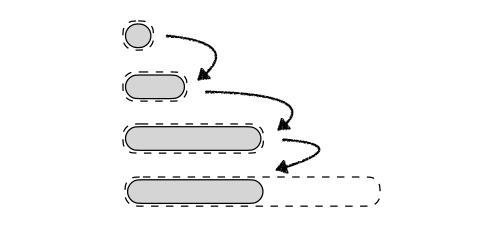
\includegraphics[width=\linewidth, height = 3cm]{full_merge.png}
  \caption{Full Merge. Reproduced from \cite{Spooky}.}
  \label{fig:spooky_results}
\end{figure}

\textbf{Partial merge} takes only one file and merges it with the files from the next level that overlap in key range, therefore makes the compaction jobs smaller, not needing so much extra space, but it increases write amplification, because the files don't overlap perfectly. This results into some entries being rewritten many times, taking as example the case in figure 2.

\begin{figure}[ht]
  \centering
  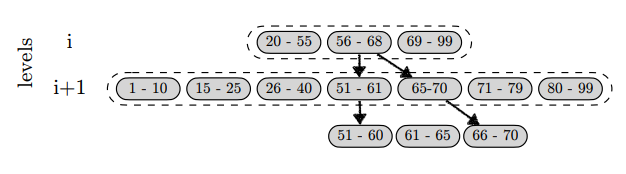
\includegraphics[width=\linewidth]{partial_merge.png}
  \caption{Partial Merge. Reproduced from \cite{Spooky}. Entries 51 - 55 and 69 - 70 rewritten because of imperfect overlap}
  \label{fig:spooky_results}
\end{figure}



\textbf{Merge Policy.} The way data is picked to be merged when the level is full can be split into two categories, leveling and tiering.\cite{Spooky} 

\textbf{Leveling} keeps a level as a single "run" and when data is merged with that level, it is merged with the entire level, resulting in a sorted distinct row of files\cite{Spooky}. The main advantage of this is that when we search for a key in a level, it can only be in one file, so we only have to read that one. Therefore it is a policy optimized for read intensive workloads.

\textbf{Tiering} splits levels into multiple runs, merging them all into one run at the next level when a level fills up. This results into no guarantee that a key cannot be in multiple runs, so when we do a lookup we have to check all runs until we find the key. If a key is not in the first run we check, we have to look in the next run that can have the key, and only when we find it the first time can we stop. As a result, it is more write optimized, as compaction jobs are smaller, since we don't merge with the entire next level.\cite{Spooky}
\begin{figure}[ht]
  \centering
  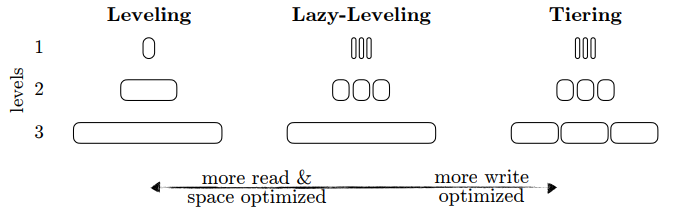
\includegraphics[width=\linewidth]{leveling_tiering.png}
  \caption{LSM-Tree merge policies. Reproduced from \cite{Spooky}. Leveling and tiering can be combined and fine-tuned, depending on the optimization goals.}
  \label{fig:spooky_results}
\end{figure}

As it can be seen in figure 3, the transition between the two policies is gradual, they do not oppose each other, but can be used in combination, to profit from the advantages of both. Lazy leveling is a result of this, making use of tiering in the first levels, that are compacted more often, so that merging doesn't take a long time. In the last level, that store the most data, it uses leveling, to be more space efficient and to make lookups faster, not storing so many duplicate entries.\cite{Spooky}

\section{Write Amplification}
Write amplification refers to the number of times an entry is rewritten to disk due to compactions or internal garbage collection of the SSD. These two multiplied result the total WA\cite{Spooky}. Write amplification is an inherent trait of the LSM-Tree because every time it compacts a level, no matter the compaction granularity or merge policy, it has to rewrite data. But these, along the size ratio T, can be optimized to yield better performance and lower write amplification, the two being strongly correlated. High WA means the "real" writes are being stalled by the rewriting of entries, bandwidth being a finite resource\cite{WiscKey}.
% Add your analysis of write amplification challenges and metrics here

\section{Problem statement} In the paper of reference (\cite{Spooky}), Dayan et al. show that the write amplification of full merge is lower than that of partial merge, not only mathematically, but also with benchmarks. Moreover, they say leveling is better for reads and tiering is better for writes. I will test these hypothesis by benchmarking RocksDB on my local setup and making comparisons with their results. 
\section{RocksDB Benchmark}
\textbf{Setup.} My machine has a 13th Gen Intel(R) Core(TM) i5-13500H CPU with 12 2.6 GHz cores, a 512 GB NVMe SSD and  16 GB of DDR5 RAM. It has a split cache architecture for the 12 cores, totaling 1.1 MB of L1, 9MB of L2 and 18 MB of L3 cache. The operating system is Ubuntu 24.04.3 LTS. An important mention is that the tests do not stress the SSD for garbage collection, as a separate SSD for the database to be stored on was not available and a partition would not stress it anyway. This affects the write amplification, making it significantly lower, but it should not affect the comparison between the different compaction granularities and merge policies, as they should all be equally affected.

\textbf{Full merge imitation.} RocksDB uses partial merge, it does not have a full merge option. However, we can choose between leveled and tiered compaction and we can also modify the minimum amount of runs needed to trigger a compaction. By setting this to a higher number while using tiered compaction we can force the database to compact an entire level at a time, transforming it into full merge. After experimenting with multiple settings, the ones that worked best were to set universal\_min\_merge\_width to 8 with compaction\_style=1 (tiered). Not only did this setup yield close results to those described in the paper from Dayan et al., but I also tracked the live size of the database while conducting the tests and I noticed sudden 2x spikes in storage utilization, as we would expect from a normal full merge while compacting the biggest level. A graph of this is not shown in this paper however, because not stressing the db for maximum disk utilization makes it look inconclusive. 

\begin{figure*}[t] % the * makes it span two columns, [t] puts it at the top
    \centering
    % Top Row
    \begin{subfigure}[b]{0.49\textwidth}
        \centering
        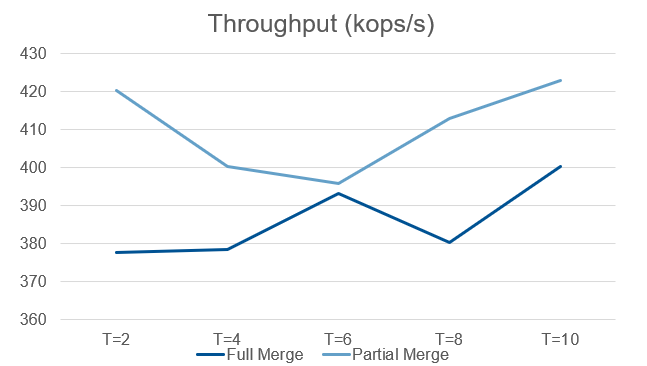
\includegraphics[width=\linewidth]{FullPartialOps.png}
        \caption{\textbf{Full Merge vs Partial Merge}}
        \label{fig:unif_partial}
    \end{subfigure}
    \hfill
    \begin{subfigure}[b]{0.49\textwidth}
        \centering
        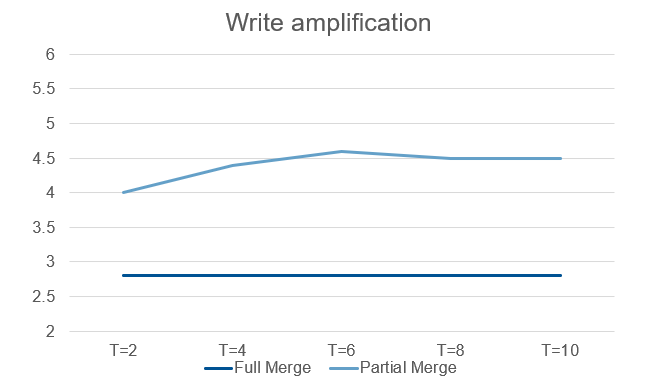
\includegraphics[width=\linewidth]{FullPartialWA.png}
        \caption{\textbf{Full Merge vs Partial Merge}}
        \label{fig:unif_full}
    \end{subfigure}
\vspace{2em}
    % Bottom Row
    \begin{subfigure}[b]{0.49\textwidth}
        \centering
        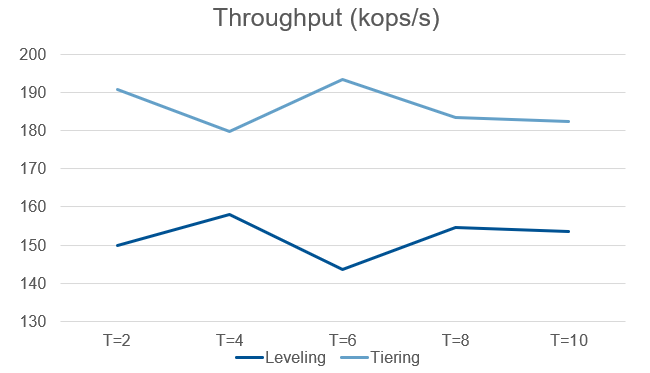
\includegraphics[width=\linewidth]{LevelingTieringOps.png}
        \caption{\textbf{Leveling vs Tiering}}
        \label{fig:skew_partial}
    \end{subfigure}
    \hfill
    \begin{subfigure}[b]{0.49\textwidth}
        \centering
        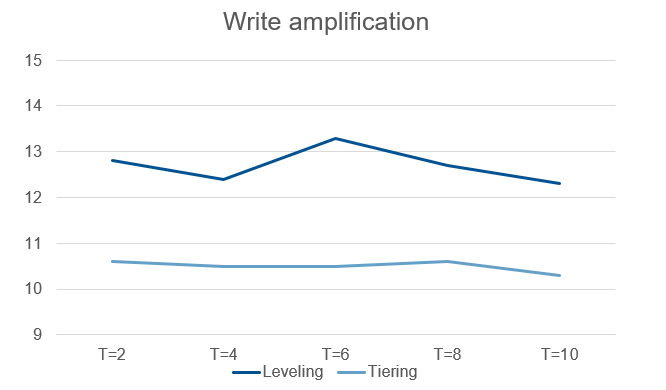
\includegraphics[width=\linewidth]{LevelingTieringWA.png}
        \caption{\textbf{Leveling vs Tiering}}
        \label{fig:skew_full}
    \end{subfigure}
    
    \caption{Comparison of Throughput and Write Amplification across compaction granularities and merge policies}
    \label{fig:grid_results}
\end{figure*}

\begin{table*}[t] 
\centering

\begin{subtable}[t]{0.49\textwidth}
    \centering
    \caption{Leveling vs Tiering}
    \begin{tabular}{|l|c|c|} 
    \hline
    \textbf{Reads} & \textbf{Leveling} & \textbf{Tiering} \\ \hline
    Uniform & 190k & 137k \\ \hline
    Skewed  & 248k  & 145k \\ \hline
    \end{tabular}
\end{subtable}
\hfill
\begin{subtable}[t]{0.49\textwidth}
    \centering
    \caption{Full Merge vs Partial Merge}
    \begin{tabular}{|l|c|c|} 
    \hline
    \textbf{Reads} & \textbf{Full Merge} & \textbf{Partial Merge} \\ \hline
    Uniform & 179k & 93k \\ \hline
    Skewed  & 180k  & 95k \\ \hline
    \end{tabular}
\end{subtable}

\vspace{10pt} % Optional: adds a bit of breathing room between tables and main caption
\caption{Read performance (Ops/sec) comparing compaction granularities and merge policies}
\label{tab:read_performance_comparison}
\end{table*}
% Add your methodology, setup, and results for the RocksDB performance tests here
\textbf{Write test}

\textbf{Full merge underperformed.} Firstly I tested full merge and partial merge while varying the size ratio. After reading the Spooky\cite{Spooky}  paper I would have expected the latter to be significantly slower than the former, but this was not the case. In figure 4 (a) we can see that partial merge outperformed full merge across all size ratios, being almost equal for T = 6. This contradicts the benchmarks in the paper of reference. 

However, when looking at write amplification (figure 4 (b)) the measurements are quite similar to those from Dayan et al. Write amplification is almost 2x as high for partial merge than for full merge. Moreover, size ratio seems to have no impact over write amplification for the latter, although it does affect throughput. Even more interesting, partial merge has both higher throughput and write amplification, which should not happen, as they should be inversely proportional. The tests were executed multiple times, under the same conditions, so the only explanation I can find is that the full merge imitation is suboptimal, as RocksDB was clearly designed with partial merge in mind. While trying different settings for the benchmark, I noticed that increasing the universal\_min\_merge\_width was yielding worse results, but it was the only way to get the database to have huge compactions, causing the 2x spikes in database size.

\textbf{Expected results for leveling and tiering.} In the Spooky\cite{Spooky} paper they emphasize that leveling is more read optimized and tiering is better for write-heavy workloads. This is also clearly highlighted in my benchmarks on RocksDB. In figure 4 (c) we can see tiering outperforming leveling in throughput across all size ratios, because it was tested on a write-only workload. When executing a compaction, it doesn't merge with the entire next level, resulting in less stalling and faster writes. 

In figure 4 (d), just as expected, we can see that tiering had a lower write amplification than leveling, hence the higher throughput. This result is not surprising, because when using tiering, the data of the full level is not merged with the next level, it is just compacted into a single run and moved to the next level, therefore not rewriting the data as many times as leveling.

\textbf{Read test}

I also tested the performance of the database for reads with the same settings. For table 1 (a) the database was first filled with random uniform writes using leveling and then tiering. When running random reads tests, just as expected, leveling performed significantly better, because it can have a single entry per level for a specific key, whereas with tiered compactions the database has to check multiple runs in a single level. With skewed reads the gap between the two only got larger, outlining the read benefits of leveling.

\textbf{Full merge performed well.} For table 1 (b) I first filled the database using full merge and then using partial merge. For each I then performed random reads tests and got results very similar to those obtained by Dayan et al. The database performed almost 2x as many reads when filled with full merge, than when using partial merge. This outcome was a bit surprising, because the full merge imitation did not perform well for writes, but actually, it goes to show that it is indeed similar to a real full mearge, just not optimal. Skewed reads yielded very similar results to uniform reads.

\textbf{Important mention}

I was not able to perform tests while combining full merge with leveling or tiering, since it is basically just partial merge with tiered compaction and very big runs. I also could not test the "Spooky"\cite{Spooky} implementation, as there is no possibility in RocksDB benchmark to choose which levels use full merge and which use partial merge. Spooky uses full preemptive merge for the first levels, and preemptive partial merge for the last 3 levels\cite{Spooky}.


 \section{Conclusion}

 Using RocksDB's benchmarking options, I was able to test the hypothesis about full and partial merge, tiering and leveling that were presented in the paper "Spooky: Granulating LSM-Tree Compactions Correctly"\cite{Spooky}. The results obtained support them, even though they were not very consistent and the full merge imitation did not perform well. It was in the end clear, that tiering is better for write-heavy workloads, while leveling is better for reads, and that full merge yields lower write amplification than partial merge.
% Add your concluding remarks and future work here

\bibliographystyle{ACM-Reference-Format}
\bibliography{sample-base}

\end{document}